% Copyright (c)  2005-2010 EDF-EADS-PHIMECA.
% Permission is granted to copy, distribute and/or modify this document
% under the terms of the GNU Free Documentation License, Version 1.2
% or any later version published by the Free Software Foundation;
% with no Invariant Sections, no Front-Cover Texts, and no Back-Cover
% Texts.  A copy of the license is included in the section entitled "GNU
% Free Documentation License".
\renewcommand{\etapemethodo}{B}
\renewcommand{\nomfichier}{docref_B231_TestPearson}
\renewcommand{\titrefiche}{Pearson's correlation test}

\Header

\MathematicalDescription{

  \underline{\textbf{Goal}} \vspace{2mm}

  This method is concerned with the modelling of a probability distribution of a random vector $\vect{X} = \left( X^1,\ldots,X^{n_X} \right)$. It seeks to find a type of dependency (here a linear correlation) which may exist between two components $X^i$ and $X^j$. \vspace{2mm}

  \underline{\textbf{Principle}} \vspace{2mm}

  The Pearson's correlation coefficient  $\rho_{U,V}$, defined in \otref{docref_B231_Pearson}{Pearson's Coefficient}, measures the strength of a linear relationship between two random variables $U$ and $V$. If we have a sample made up of $N$ pairs $\left\{ (u_1,v_1),(u_2,v_2),(u_N,v_N) \right\}$, we denote $\widehat{\rho}_{U,V}$  to be the estimated coefficient.

  Even in the case where two variables $U$ and $V$ have a Pearson's coefficient  $\rho_{U,V}$ equal to zero, the estimate  $\widehat{\rho}_{U,V}$ obtained from the sample may be non-zero: the limited sample size does not provide the perfect image of the real correlation. Pearson's test nevertheless enables one to determine if the value obtained by $\widehat{\rho}_{U,V}$ is significantly different from zero. More precisely, the user first chooses a probability $\alpha$. From this value the critical value $d_\alpha$  is calculated such that:
  \begin{itemize}
  \item         if $\left| \widehat{\rho}_{U,V} \right| > d_\alpha$, one can conclude that the real Pearson's correlation coefficient $\rho_{U,V}$   is not zero; the risk of error in making this assertion is controlled and equal to $\alpha$;
  \item if $\left| \widehat{\rho}_{U,V} \right| \leq d_\alpha$, there is insufficient evidence to reject the null hypothesis $\rho_{U,V} = 0$.
  \end{itemize}

  An important notion is the so-called "$p$-value" of the test. This quantity is equal to the limit error probability $\alpha_\textrm{lim}$ under which the null correlation hypothesis is rejected. Thus, Pearson's coefficient is supposed non zero if and only if $\alpha_\textrm{lim}$ is greater than the value $\alpha$ desired by the user. Note that the higher $\alpha_\textrm{lim} - \alpha$, the more robust the decision.

  \begin{center}
    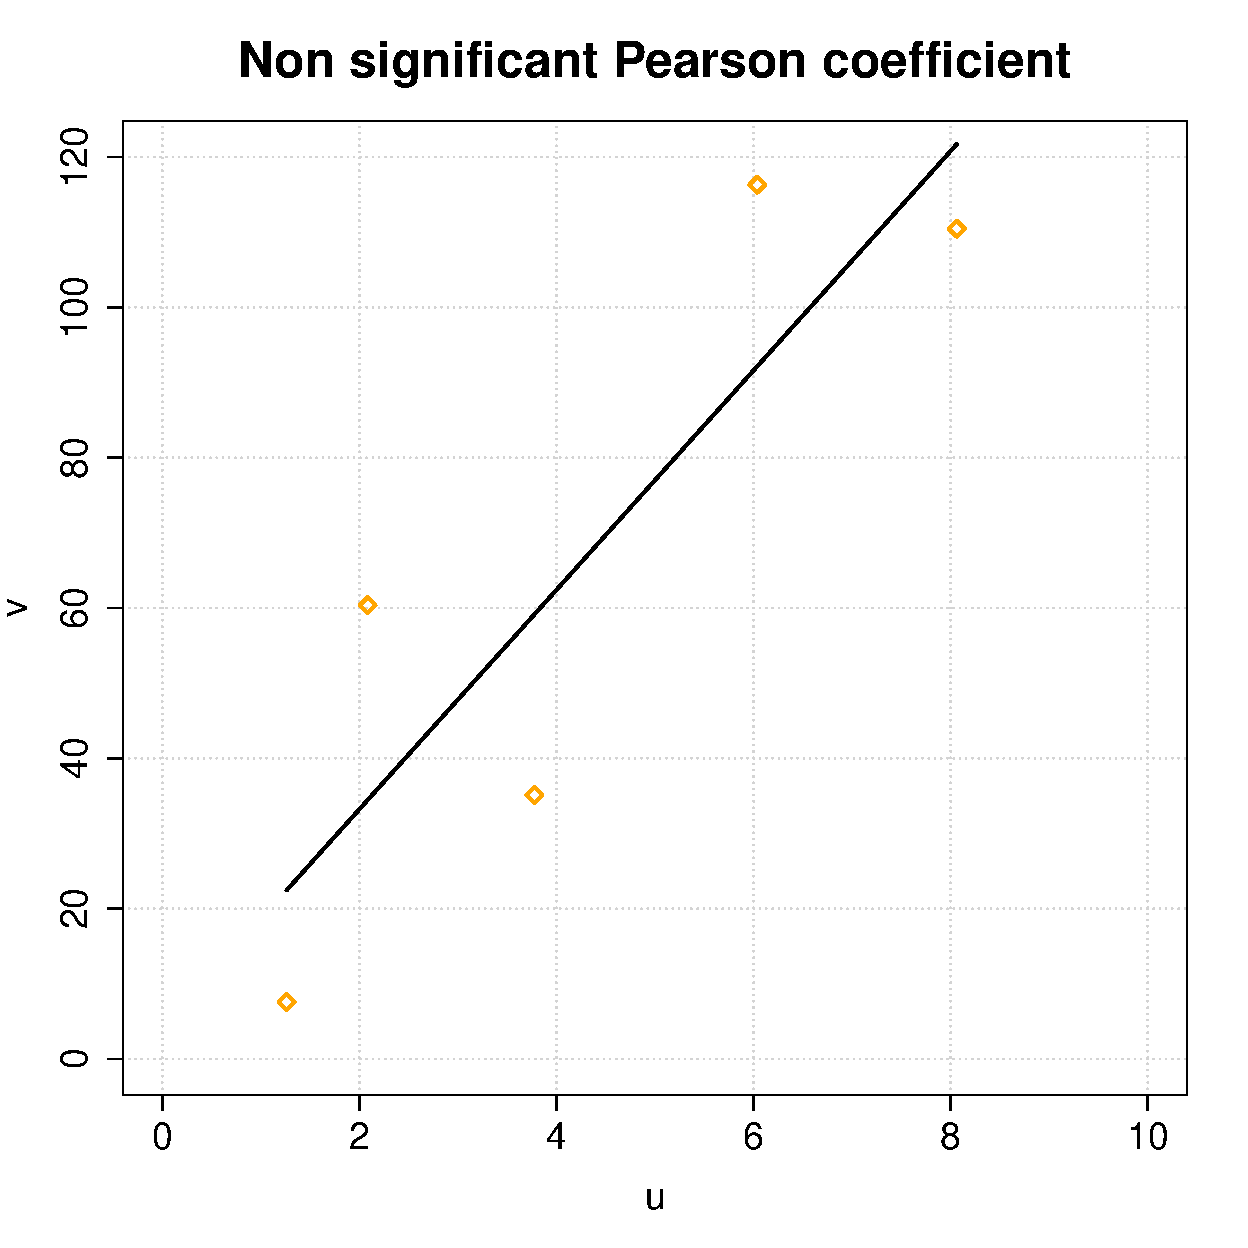
\includegraphics[width=0.5\textwidth]{pearson2.pdf}
  \end{center}

}
{
  -
}

\Methodology{
  The Pearson's test is used in step B "Quantifying Sources of Uncertainty". It enables us to verify if a linear type of dependency exists between the two components $X^i$ and $X^j$ of the input variable vector $\underline{X}$ defined in step A "Specifying Criteria and the Case Study". Such a relationship should in fact be taken into account to avoid distortion of results in step C "Propagation of Uncertainty".

  {\bf Input data~:}\\
  Two samples $\left\{ x^i_1,\ldots,x^i_N \right\}$  and $\left\{ x^j_1,\ldots,x^j_N \right\}$  of variables $X^i$ and $X^j$, each pair $\left( x^i_k,x^j_k \right)$  corresponding to a simultaneous sampling of the two variables

  {\bf Parameters~:}\\
  a probability $\alpha$ taking values strictly between 0 and 1, defining the risk of permissible decision error (significance level)

  {\bf Outputs~:}\\
  $Result$ : Binary variable specifying whether the hypothesis of a correlation coefficient equal to 0 is rejected (0) or not (1) \\
  $\alpha_\textrm{lim}$ : $p$-value of the test}
{
  Certain precautions should be taken when interpreting the Pearson's test results.
  \begin{itemize}
  \item The underlying theory of the Pearson test assumes in fact that the variables $X^i$ and $X^j$ are both normally distributed. In all other cases, the decision produced by the test is only valid if the sample size $N$ is sufficiently large (in practice $N \geq$ a few dozen, even if there is no theoretical result that enables us to prove that asymptotic behaviour has been attained).
  \item Still considering the case of distributions other than the Normal distribution, whatever the value of $N$, we recall that  $\rho_{X^i,X^j}= 0$ does not enable us to conclude that $X^i$ and $X^j$ are independent (see \otref{docref_B231_Pearson}{Pearson's Correlation Coefficient}).
  \item More generally, the numerical value of Pearson's correlation coefficient can only be interpreted when the two variables studied $X^i$ and $X^j$ are related in a linear way; the scatter plot of points $\left\{ (x^i_1,x^j_1),\ldots,(x^i_N,x^j_N) \right\}$  provides some indication concerning the validity of this hypothesis.
  \end{itemize}

  The following pages describe methods which enable us to test the hypothesis of the Normal distribution using the available sample $\left\{ x^i_1,\ldots,x^i_N \right\}$ and $\left\{ x^j_1,\ldots,x^j_N \right\}$: \otref{docref_B222_TestKS}{Kolmogorov-Smirnov Goodness of Fit Test},
  \otref{docref_B222_TestCVM}{Cramer-von Mises Goodness of Fit Test}, \otref{docref_B222_TestAD}{Anderson-Darling Goodness of Fit Test}.

  Out of Pearson's test validity domain (i.e. linear relationship, Normal distributions), \otref{docref_B232_TestSpearman}{Spearman's test} provides some answers.

  The following bibliographical references provide main starting points for further study of this method:
  \begin{itemize}
  \item Saporta, G. (1990). "Probabilités, Analyse de données et Statistique", Technip
  \item Dixon, W.J. \& Massey, F.J. (1983) "Introduction to statistical analysis (4th ed.)", McGraw-Hill
    % \item NIST/SEMATECH e-Handbook of Statistical Methods, http://www.itl.nist.gov/div898/handbook/
    % \item D'Agostino, R.B. and Stephens, M.A. (1986). "Goodness-of-Fit Techniques", Marcel Dekker, Inc., New York.
  \item Bhattacharyya, G.K., and R.A. Johnson, (1997). "Statistical Concepts and Methods", John Wiley and Sons, New York.
    % \item Sprent, P., and Smeeton, N.C. (2001). "Applied Nonparametric Statistical Methods -- Third edition", Chapman \& Hall
    % \item Burnham, K.P., and Anderson, D.R (2002). "Model Selection and Multimodel Inference: A Practical Information Theoretic Approach", Springer
  \end{itemize}
}
